\hypertarget{Introduction}{%
\section{Introduction}\label{Introduction}}

\begin{figure}[htpb]
    \centering
    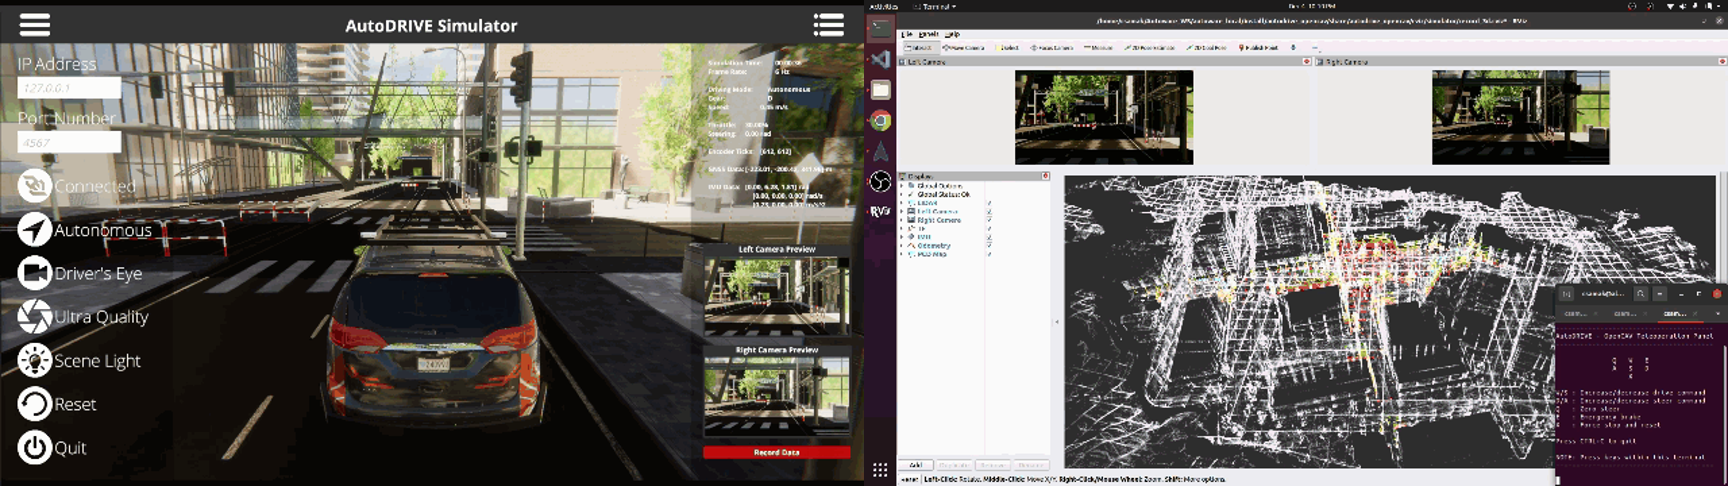
\includegraphics[width=\linewidth]{Figures/fig1.png}
    \caption{Project overview demonstrating the integration of AutoDRIVE Ecosystem with Autoware stack for the application of autonomous valet parking using the OpenCAV.}
    \label{fig: figure1}
\end{figure}

\hypertarget{Motivation}{%
\subsection{Motivation}\label{Motivation}}

Modeling and simulation of autonomous vehicles plays a crucial role in achieving enterprise-scale realization that aligns with technical, business and regulatory requirements. Contemporary trends in digital lifecycle treatment have proven beneficial to support simulation-based-design (SBD) as well as verification and validation of increasingly complex systems and system-of-systems. However, the development of appropriate fidelity simulation models capable of capturing the intricate real-world physics and graphics (real2sim), while enabling real-time interactivity for decision-making, has remained a challenge.

Autonomy-oriented simulations, as opposed to conventional simulations, must equally prioritize back-end physics and front-end graphics, which is crucial for realistic simulation of vehicle dynamics, sensor characteristics, and environmental physics. Additionally, the interconnect between vehicles, sensors, actuators and the environment, along with peer vehicles and infrastructure in a scene must be appropriately modeled. Most importantly, however, these simulations should allow real-time interfacing with software development framework(s) to support reliable verification and validation of autonomy algorithms.

Recent advances in AI-based tools and workflows, such as online deep-learning algorithms leveraging live-streaming data sources, offer the tantalizing potential for real-time system-identification and adaptive modeling to simulate vehicle(s), environment(s), as well as their interactions. This transition from static/fixed-parameter ``virtual prototypes'' to dynamic/adaptable ``digital twins'' not only improves simulation fidelity and real-time factor, but can also support the development of online adaption/augmentation techniques that can help bridge the gap between simulation and reality (sim2real).

However, seamlessly moving from reality to simulation and back to reality (real2sim2real) \cite{Real2Sim2Real} requires a sleek workflow in place. In such a milieu, this work focuses on developing autonomy-oriented digital twins of vehicles across different scales and configurations to help support the streamlined development and deployment of Autoware Core/Universe stack \cite{AutowareCore, AutowareUniverse, AutowareStack}, using a unified real2sim2real toolchain. Needless to say, these ``autonomy-oriented'' digital twins, as opposed to conventional simulation models, prioritize equal detailing of physics and graphics.

\hypertarget{Objectives}{%
\subsection{Objectives}\label{Objectives}}

The core deliverable of this project was integrating Autoware\footnote{\url{https://autoware.org}} \cite{Autoware} stack with AutoDRIVE Ecosystem\footnote{\url{https://autodrive-ecosystem.github.io}} \cite{AutoDRIVEEcosystem, AutoDRIVESimulator, AutoDRIVEReport, AutoDRIVESimulatorReport} to demonstrate the end-to-end task of mapping an unknown environment, recording a trajectory within the mapped environment, and autonomously tracking the pre-recorded trajectory to achieve the desired objective (Fig. \ref{fig: figure1}). Particularly, we demonstrate sim2real Autoware deployments using Nigel \cite{Nigel} and F1TENTH \cite{F1TENTH}, two small-scale autonomous vehicle platforms with unique qualities and capabilities. Additionally we demonstrate simulated Autoware deployments using mid-scale Hunter SE \cite{HunterSE} and full-scale OpenCAV \cite{OpenCAV} within simplistic and realistic scenarios. It is worth mentioning that this study describes the first-ever off-road deployment of the Autoware stack using the mid-scale vehicle platform, thereby expanding the operational design domain (ODD) of Autoware beyond on-road autonomous navigation.

As a precursor to Autoware deployments, this work discusses the development of vehicle and environment digital twins using AutoDRIVE Ecosystem, which span across different scales and operational design domains. The development of these autonomy-oriented digital twins was, therefore, the secondary objective of this project. This step involved developing geometric as well as dynamics models of vehicles and calibrating them against their real-world counterparts. Additionally, developing physics-based models for interoceptive as well as exteroceptive sensors and actuators was accomplished based on their respective datasheets. Finally, creating physically and graphically realistic on-road and off-road environments across scales marked the completion of this objective.

The tertiary objective of this project was to develop cross-platform application programming interfaces (APIs) and human-machine interfaces (HMIs) to connect with AutoDRIVE Ecosystem, which would aid in AutoDRIVE-Autoware integration. This objective, in conjunction with the secondary objective enabled the realization of the primary objective of developing a streamlined real2sim2real autoware development framework with deployment demonstrations across varying scales and ODDs.

\hypertarget{Applications}{%
\subsection{Applications}\label{Applications}}

Following is a brief summary of the potential applications and scope of this project, which align well with the different ODDs and use cases of Autoware Foundation \cite{AutowareOverview}:

\begin{itemize}
    \item \textbf{Autonomous Valet Parking (AVP)}: Mapping of a parking lot, localization within the created map and autonomous driving within the parking lot.
    \item \textbf{Cargo Delivery}: Autonomous mobile robots for the transport of goods between multiple points or last-mile delivery.
    \item \textbf{Racing}: Autonomous racing using small-scale (e.g. F1TENTH) and full-scale (e.g. Indy Autonomous Challenge \cite{IAC}) vehicles running the Autoware stack.
    \item \textbf{Robo-Bus/Shuttle}: Fully autonomous (Level 4) buses and shuttles operating on public roads with predefined routes and stops.
    \item \textbf{Robo-Taxi}: Fully autonomous (Level 4) taxis operating in dense urban environments to pick-up and drop passengers from point-A to point-B.
    \item \textbf{Off-Road Exploration}: Although the Autoware Foundation has not yet proposed such an ODD, this study describes the first-ever off-road deployment of the Autoware stack using the mid-scale vehicle platform, thereby expanding the operational design domain (ODD) of Autoware beyond on-road autonomous navigation. Such off-road deployments could be applied for agricultural, military or extra-terrestrial applications.
\end{itemize}
